% chap6.tex

\chapter{Augmented Reality}\label{chap:ar}
Augmented Reality is artificial computer generated stimuli which is overlaid onto physical world. It differs from Virtual Reality in a way that it does not suppress perception of physical world but mixes physical reality with virtual content.


A general procedure to generate augmented reality content is described below.
\begin{enumerate}
	\item \textbf{Initialize camera} - This is to capture the real world content.
	\item \textbf{Capture} - The captured real world content is processed to identify pre-defined patterns.
	\item \textbf{Identify Marker} - Marker is a predefined pattern available within applications database. Image Processing techniques are used to recognize the presence of marker in the captured video feed.
	\item \textbf{Retrieving Position/Orientation} - Once the marker is recognized, the position and orientation of the marker is identified and given to the application.
	\item \textbf{Render Object} - The application renders the virtual content using the position and orientation information got from the above step.
	\item \textbf{Augment} - In this step the virtual content is layered over the real content.
\end{enumerate}

Figure~\ref{fig:ar} illustrates these steps.

\begin{figure}[h]
\centering
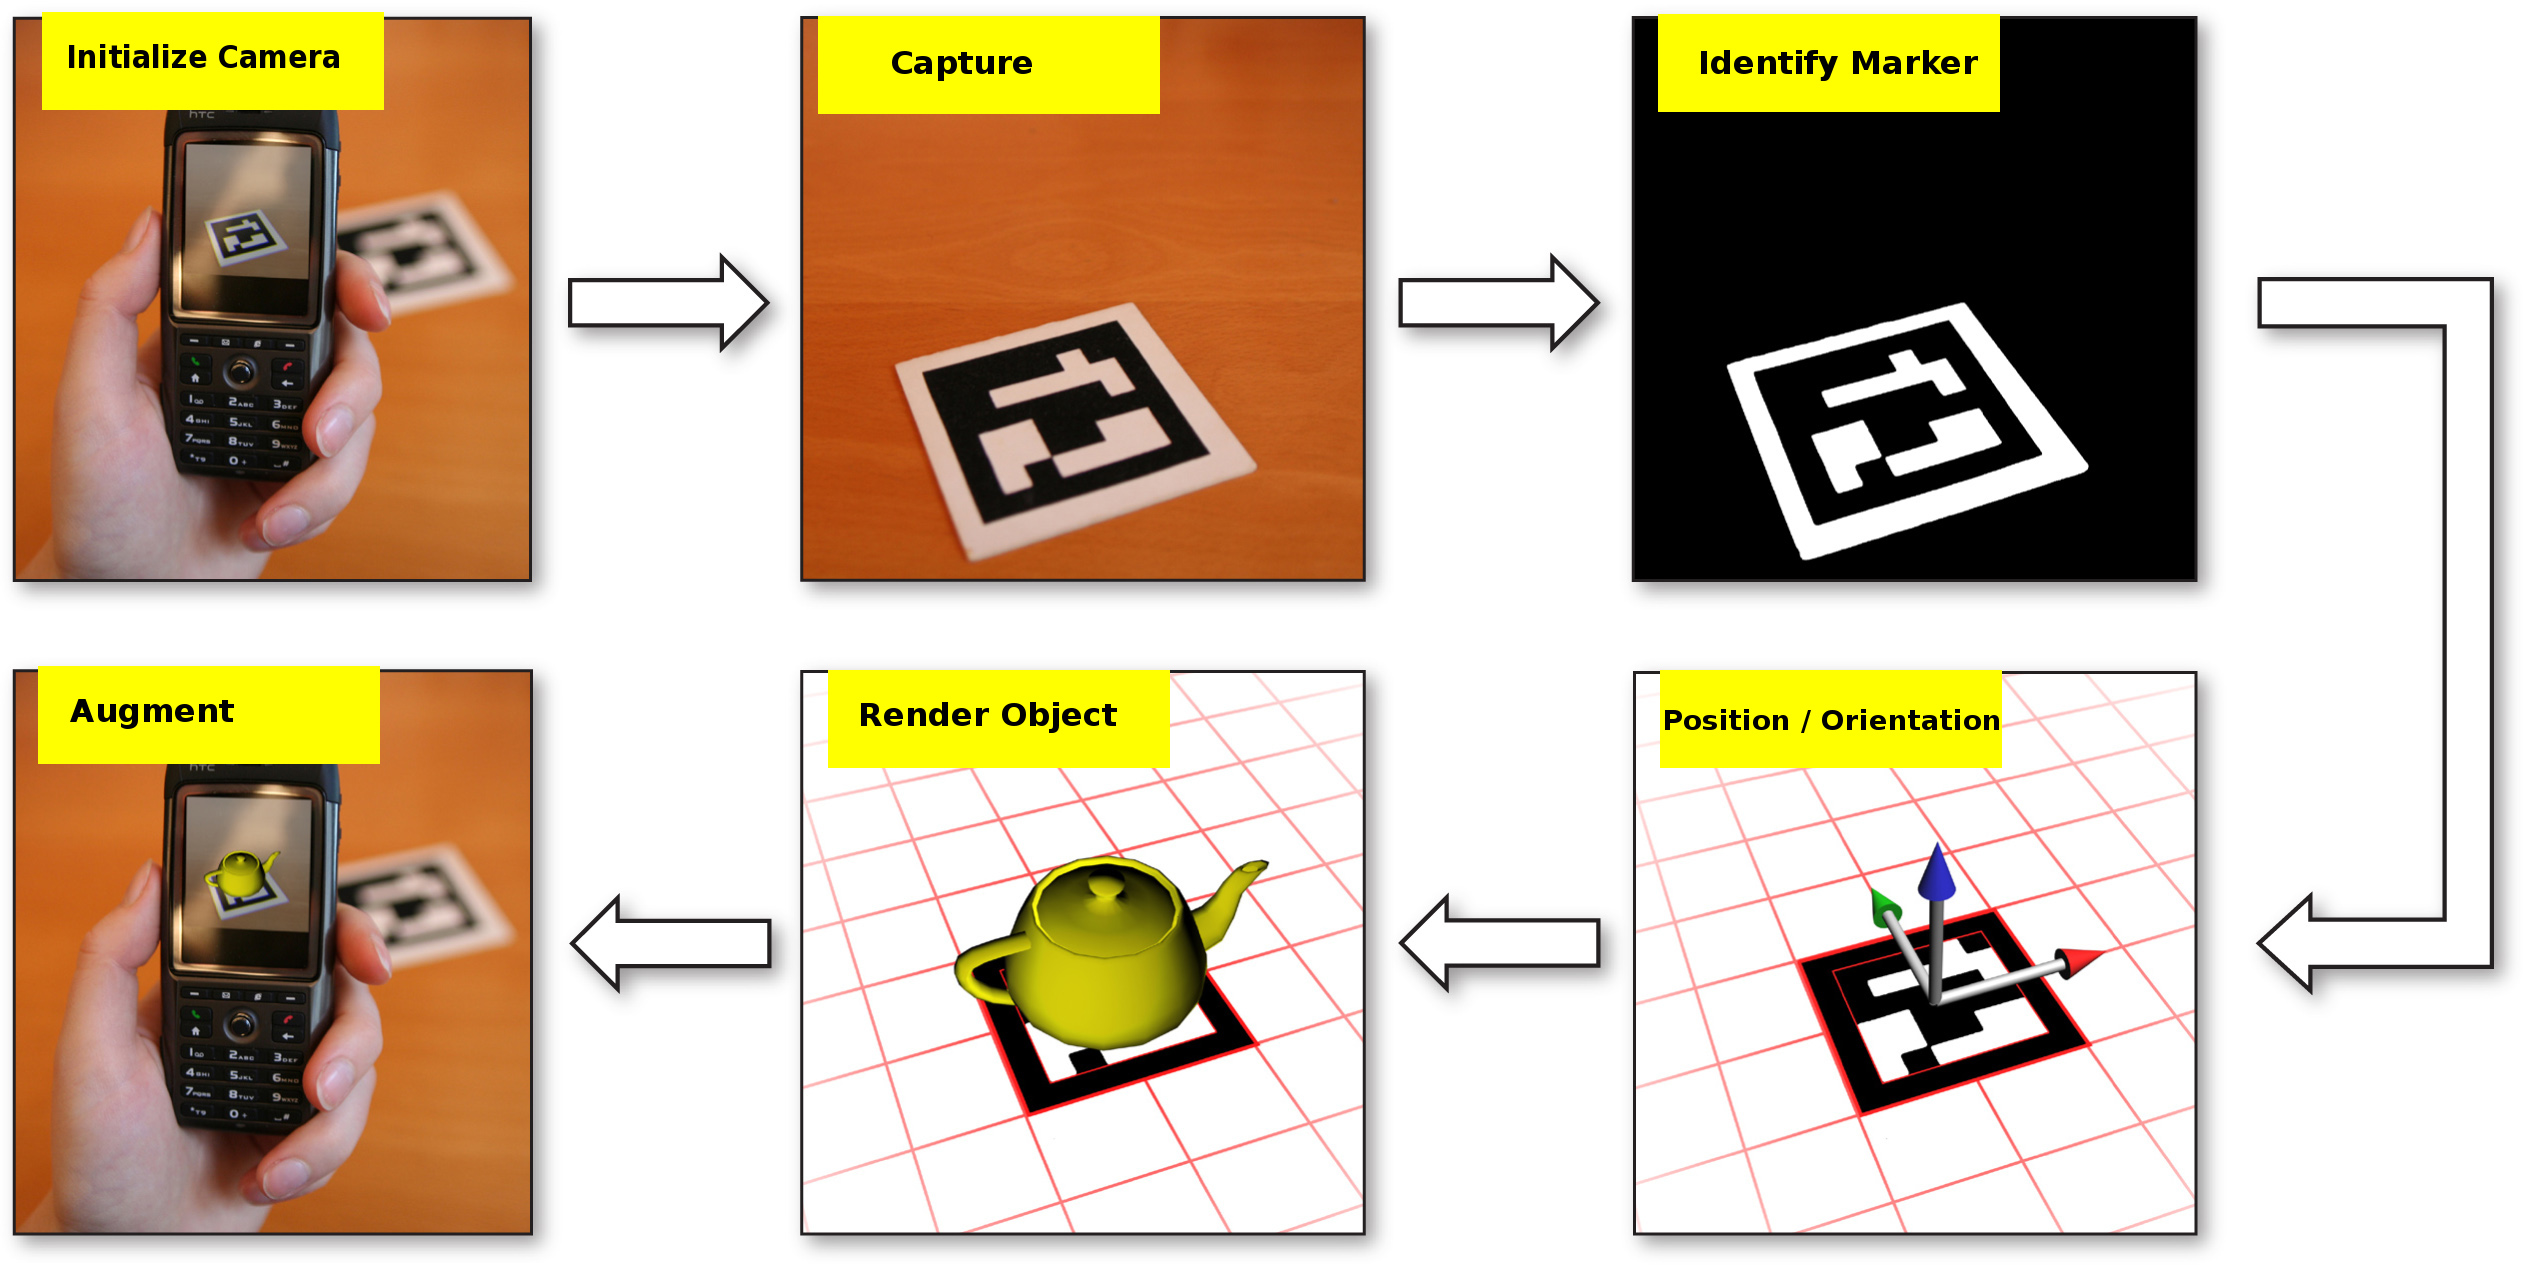
\includegraphics[width=1\columnwidth]{Images/marker_tracking}
\caption{Steps to generated AR content}
\label{fig:ar}
\end{figure}

\section{Vuforia Augmented Reality SDK}
Vuforia is an Augmented Reality Software Development Kit (SDK) for mobile devices that enables the creation of Augmented Reality applications. It uses Computer Vision technology to recognize and track planar images (Image Targets) and simple 3D objects, such as boxes, in real-time. This image registration capability enables developers to position and orient virtual objects, such as 3D models and other media, in relation to real world images when these are viewed through the camera of a mobile device. The virtual object then tracks the position and orientation of the image in real-time so that the viewer’s perspective on the object corresponds with their perspective on the Image Target, so that it appears that the virtual object is a part of the real world scene.

\section{Vuforia SDK Configuration}
Vuforia SDK can be downloaded from https://developer.vuforia.com/downloads/sdk. To configure the SDK with Android Studio below steps were followed.
\begin{itemize}
\item Launch Android Studio
\item Select File - Import Project and browse to the root directory of the Vuforia project you want to open
\item Proceed in the Import Wizard dialog (click Next, Next) until you reach a page with this message "Alternatively, you can fill in the actual path map in the table below":
\item Click to edit
\item Enter the actual path to the Vuforia.jar library
\item In the Project view, right-click on the Project and expand the view hierarchy so to locate the Vuforia.jar under "app/src/main"
\item Right-click on Vuforia.jar to open the context menu
\item click on the "Add as library..." option in the context menu
\item Alternatively, if you cannot locate the Vuforia.jar in your project hierarchy right-click on the Project and select "Open Module Settings", select "App", then select the "Dependencies" tab and click on the "+" button to Add a File Dependency and browse to the Vuforia.jar file
\item Create a folder called "jniLibs" under the "app/src/main" folder under your Android Studio project directory
\item Copy the "armeabi-v7a" folder (including the libVuforia.so file located inside it) from the "installdir/build/lib" to the "app/src/main/jniLibs" folder
\item the resulting directory structure under your project root should be "/app/src/main/jniLibs/armeabi-v7a/libVuforia.so"
\item Clean and rebuild the project
\item Run the app on your device
\end{itemize}

\section{Creating the virtual content}
The virtual content was created using a 3D modeling tool, Autodesk Maya. The process involved 3 steps - 
\begin{enumerate}
\item 3D Modeling
\item Texture Mapping
\item Exporting the 3D Model
\end{enumerate}

\subsection{3D Modeling}
3D modeling (or modelling) is the process of developing a mathematical representation of any three-dimensional surface of an object via specialized software. The outcome is called a 3D model. It can be displayed as a two-dimensional image through a process called 3D rendering or it can be used for simulation purposes. The 3D model of the robot created is shown in Figure~\ref{fig:model}

\begin{figure}[h]
\centering
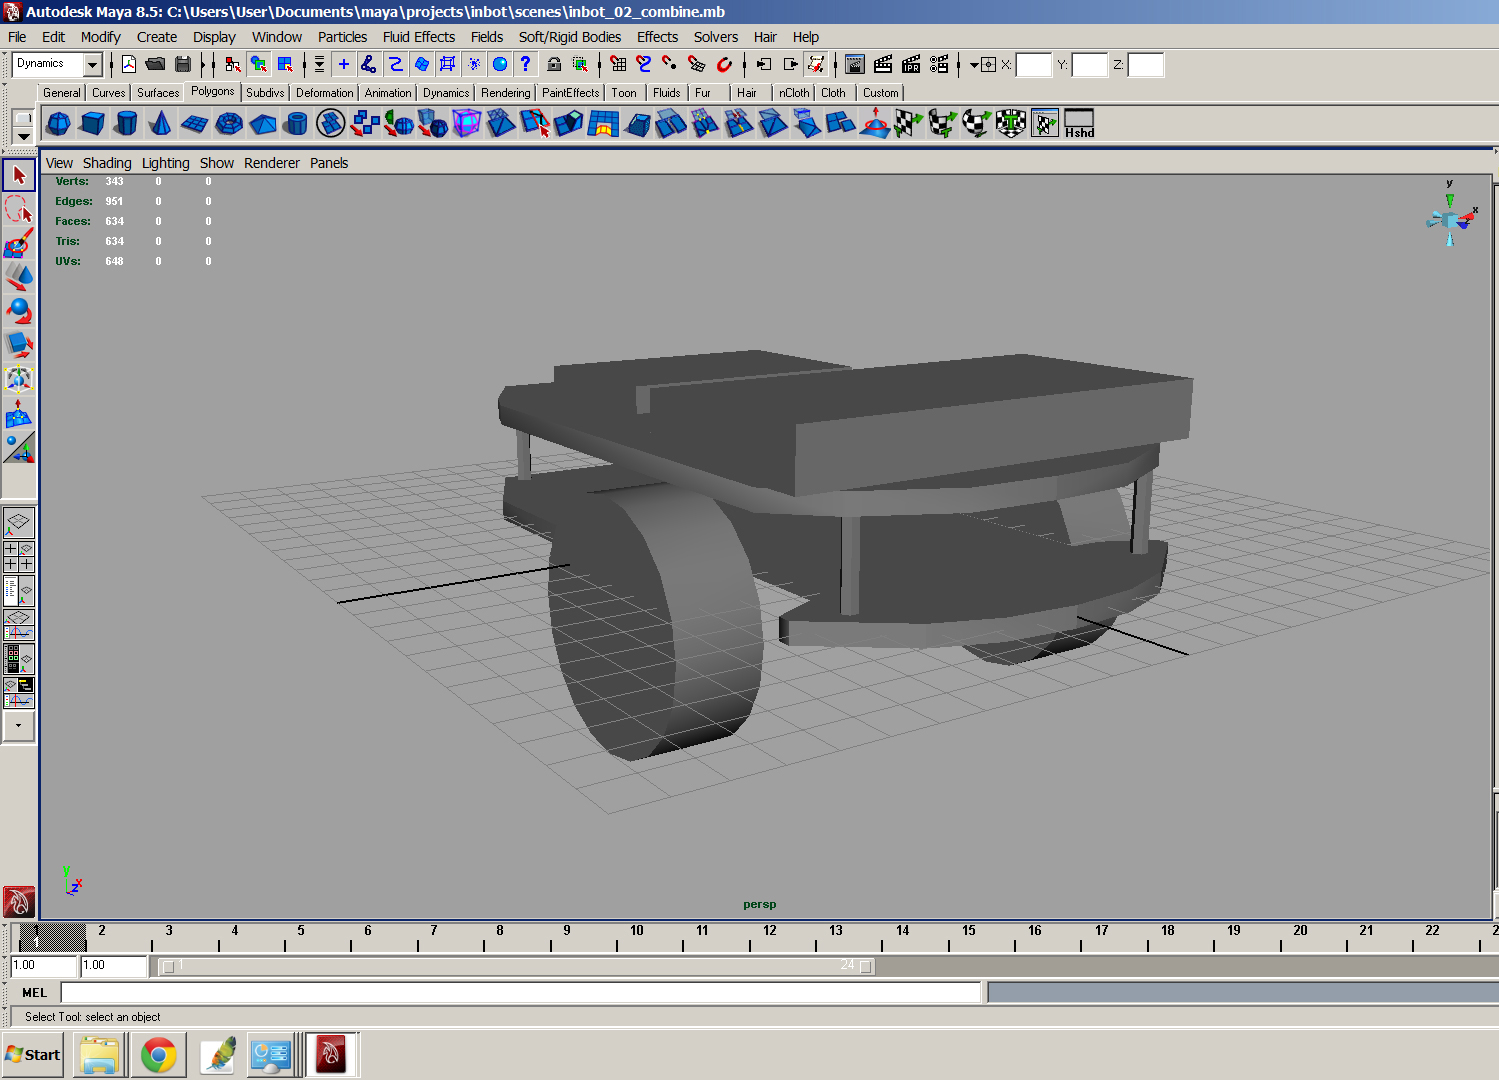
\includegraphics[width=1\columnwidth]{Images/model}
\caption{3D model created in Maya}
\label{fig:model}
\end{figure}

\subsection{Texture Mapping}

Texture mapping is a method for adding detail, surface texture (a bitmap or raster image), or color to a computer-generated graphic or 3D model. A texture map is applied (mapped) to the surface of a shape or polygon. This process is akin to applying patterned paper to a plain white box. Every vertex in a polygon is assigned a texture coordinate which in the 2d case is also known as a UV coordinate. Image sampling locations are then interpolated across the face of a polygon to produce a visual result that seems to have more richness than could otherwise be achieved with a limited number of polygons. The texture map used for the 3D model and the texture mapped 3D model is shown in Figure-\ref{fig:texture_map} and Figure~\ref{fig:texture_mapped_model} respectively.

\begin{figure}[h]
\centering
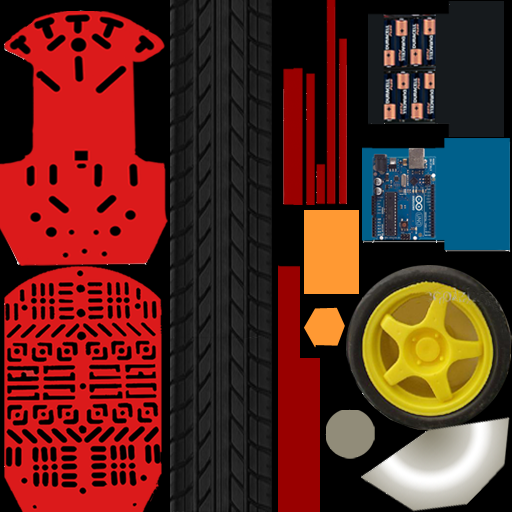
\includegraphics[width=0.6\columnwidth]{Images/texture_map}
\caption{Texture Map created using Photoshop}
\label{fig:texture_map}
\end{figure}

\begin{figure}[h]
\centering
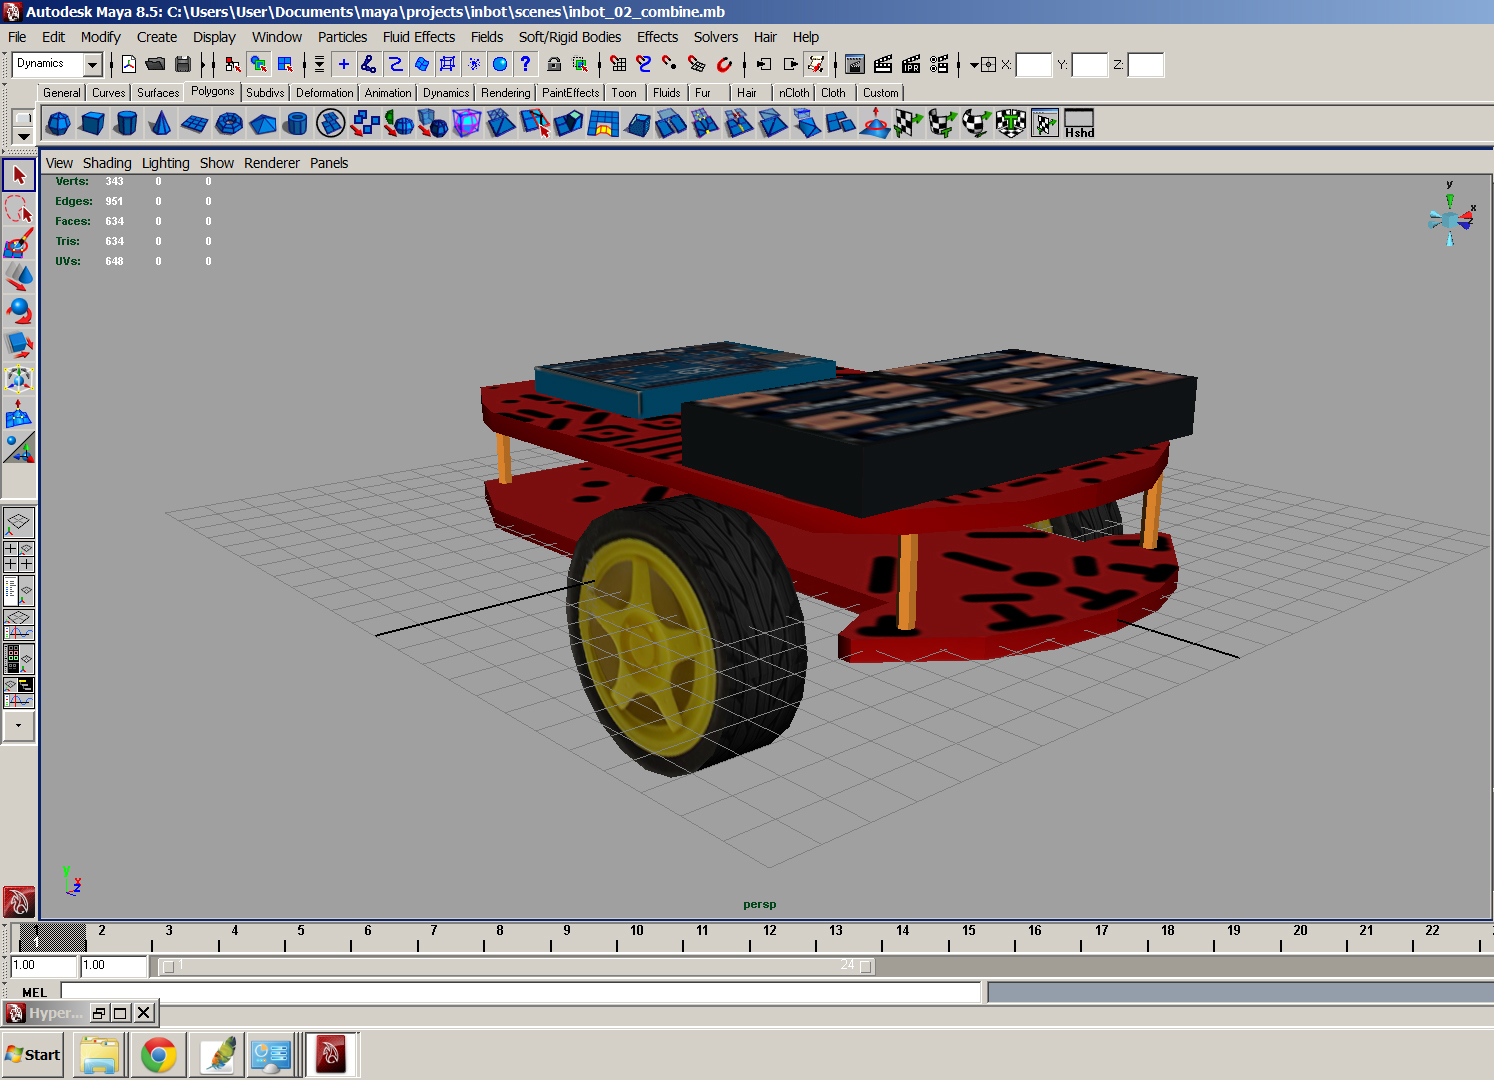
\includegraphics[width=1\columnwidth]{Images/textured_model}
\caption{Texture Mapped model in Maya}
\label{fig:texture_mapped_model}
\end{figure}

\subsection{Exporting the 3D Model}
Once the model was textured mapped, it was exported to OBJ file format. OBJ file format is a simple data-format that represents 3D geometry using the position of each vertex, the UV position of each texture coordinate vertex, vertex normals, and the faces that make each polygon defined as a list of vertices, and texture vertices. This information was using in Android platform to recreate the virtual content.